%
% Anwendung: Gauss-Quadratur
%
\section{Anwendung: Gauss-Quadratur}
\rhead{Gauss-Quadratur}
Orthogonale Polynome haben eine etwas unerwartet Anwendung in einem
von Gauss erdachten numerischen Integrationsverfahren.
Es basiert auf der Beobachtung, dass viele Funktionen sich sehr
gut durch Polynome approximieren lassen.
Wenn man also sicherstellt, dass ein Verfahren für Polynome
sehr gut funktioniert, darf man auch davon ausgehen, dass es für
andere Funktionen nicht allzu schlecht sein wird.

\subsection{Interpolationspolynome}
Zu einer stetigen Funktion $f(x)$ auf dem Intervall $[-1,1]$ 
ist ein Polynome vom Grad $n$ gesucht, welches in den Punkten
$x_0<x_1<\dots<x_n$ die Funktionswerte $f(x_i)$ annimmt.
Ein solches Polynom $p(x)$ hat $n+1$ Koeffizienten, die aus dem
linearen Gleichungssystem der $n+1$ Gleichungen $p(x_i)=f(x_i)$ 
ermittelt werden können.

Das Interpolationspolynom $p(x)$ lässt sich abera uch direkt 
angeben.
Dazu konstruiert man zuerst die Polynome
\[
l_i(x)
=
\frac{
(x-x_0)(x-x_1)\cdots\widehat{(x-x_i)}\cdots (x-x_n)
}{
(x_i-x_0)(x_i-x_1)\cdots\widehat{(x_i-x_i)}\cdots (x_i-x_n)
}
\]
vom Grad $n$, wobei der Hut bedeutet, dass diese Faktoren
im Produkt wegzulassen sind.
Die Polynome $l_i(x)$ haben die Eigenschaft
\[
l_i(x_j) = \delta_{ij}
=
\begin{cases}
1&\qquad i=j\\
0&\qquad\text{sonst}.
\end{cases}
\]
Die Linearkombination
\[
p(x) = \sum_{i=0}^n f(x_i)l_i(x)
\]
ist dann ein Polynom vom Grad $n$, welches am den Stellen $x_j$
die Werte
\[
p(x_j) 
=
\sum_{i=0}^n f(x_i)l_i(x_j)
=
\sum_{i=0}^n f(x_i)\delta_{ij}
=
f(x_j)
\]
hat, das Polynome $p(x)$ ist also das gesuchte Interpolationspolynom.

\subsection{Integrationsverfahren auf der Basis von Interpolation}
Das Integral einer stetigen Funktion $f(x)$ auf dem Intervall $[-1,1]$
kann mit Hilfe des Interpolationspolynoms approximiert werden.
Wenn $|f(x)-p(x)|<\varepsilon$ ist im Intervall $[-1,1]$, dann gilt
für die Integrale
\[
\biggl|\int_{-1}^1 f(x)\,dx -\int_{-1}^1p(x)\,dx\biggr|
\le
\int_{-1}^1 |f(x)-p(x)|\,dx
\le
2\varepsilon.
\]
Ein Interpolationspolynom mit kleinem Fehler liefert also auch
eine gute Approximation für das Integral.

Da das Interpolationspolynome durch die Funktionswerte $f(x_i)$
bestimmt ist, muss auch das Integral allein aus diesen Funktionswerten
berechnet werden können.
Tatsächlich ist
\begin{equation}
\int_{-1}^1 p(x)\,dx
=
\int_{-1}^1 \sum_{i=0}^n f(x_i)l_i(x)\,dx
=
\sum_{i=0}^n f(x_i)
\underbrace{\int_{-1}^1
l_i(x)\,dx}_{\displaystyle = A_i}.
\label{buch:integral:gaussquadratur:eqn:Aidef}
\end{equation}
Das Integral von $f(x)$ wird also durch eine mit den Zahlen $A_i$
gewichtete Summe
\[
\int_{-1}^1 f(x)\,dx
\approx
\sum_{i=1}^n f(x_i)A_i
\]
approximiert.

\subsection{Integrationsverfahren, die für Polynome exakt sind}
Ein Polynom vom Grad $2n$ hat $2n+1$ Koeffizienten.
Um das Polynom durch ein Interpolationspolynom exakt wiederzugeben,
braucht man $2n+1$ Stützstellen.
Andererseits gilt
\[
\int_{-1}^1 a_{2n}x^{2n} + a_{2n-1}x^{2n-1} + \dots + a_2x^2 + a_1x + a_0\,dx
=
\int_{-1}^1 a_{2n}x^{2n} + a_{2n-2}x^{2n-2}+\dots +a_2x^2 +a_0\,dx,
\]
das Integral ist also bereits durch die $n+1$ Koeffizienten mit geradem
Index bestimmt.
Es sollte daher möglich sein, aus $n+1$ Funktionswerten eines beliebigen
Polynoms vom Grad höchstens $2n$ an geeignet gewählten Stützstellen das
Integral exakt zu bestimmen.

\begin{beispiel}
Wir versuchen dies für quadratische Polynome durchzuführen, also 
für $n=1$.
Gesucht sind also zwei Werte $x_i$, $i=0,1$ und Gewichte $A_i$, $i=0,1$
derart, dass für jedes quadratische Polynome $p(x)=a_2x^2+a_1x+a_0$ 
das Integral durch
\[
\int_{-1}^1 p(x)\,dx
=
A_0 p(x_0) + A_1 p(x_1)
\]
gebeben ist.
Indem wir für $p(x)$ die Polynome $1$, $x$, $x^2$ und $x^3$ einsetzen,
erhalten wir vier Gleichungen
\[
\begin{aligned}
p(x)&=\rlap{$1$}\phantom{x^2}\colon& 2       &= A_0\phantom{x_0}+ A_1     \\
p(x)&=x^{\phantom{2}}\colon& 0       &= A_0x_0   + A_1x_1  \\
p(x)&=x^2\colon& \frac23 &= A_0x_0^2 + A_1x_1^2\\
p(x)&=x^3\colon& 0       &= A_0x_0^3 + A_1x_1^3.
\end{aligned}
\]
Dividiert man die vierte durch die zweite Gleichung in der Form
\[
\left.
\begin{aligned}
A_0x_0^3 &= -A_1x_1^3 &\qquad&\text{(vierte Gleichung)}\\
A_0x_0   &= -A_1x_1   &\qquad&\text{(zweite Gleichung)}
\end{aligned}
\quad
\right\}
\quad
\Rightarrow
\quad
x_0^2=x_1^2
\quad
\Rightarrow
\quad
x_1=-x_0.
\]
Indem wir dies in die zweite Gleichung einsetzen, finden wir 
\[
0 = A_0x_0 + A_1x_1 = A_0x_0 -A_1x_0 = (A_0-A_1)x_0
\quad\Rightarrow\quad
A_0=A_1.
\]
Aus der ersten Gleichung folgt jetzt
\[
2= A_0+A_1 = 2A_0 \quad\Rightarrow\quad A_0 = 1.
\]
Damit bleiben nur noch die Werte von $x_i$ zu bestimmen, was 
mit Hilfe der zweiten Gleichung geschehen kann:
\[
\frac23 = A_0x_0^2 + A_1x_1^2 = 2x_0^2
\quad\Rightarrow\quad
x_0 = \frac{1}{\sqrt{3}}, x_1 = -\frac{1}{\sqrt{3}}
\]
Damit ist das Problem gelöst: das Integral eines Polynoms vom Grad 3
im Interval $[-1,1]$ ist exakt gegeben durch
\[
\int_{-1}^1 p(x)\,dx
=
p\biggl(-\frac{1}{\sqrt{3}}\biggr)
+
p\biggl(\frac{1}{\sqrt{3}}\biggr).
\]
Das Integral kann also durch nur zwei Auswertungen des Polynoms
exakt bestimmt werden.

Im Laufe der Lösung des Gleichungssystems wurden die Gewichte $A_i$
mit bestimmt.
Es ist aber auch möglich, die Gewichte zu bestimmen, wenn man die
Stützstellen kennt.
Nach \eqref{buch:integral:gaussquadratur:eqn:Aidef}
sind sie die $A_i$ gegeben als Integrale der Polynome
$l_i(x)$, die im vorliegenden Fall linear sind:
\begin{align*}
l_0(x)
&=
\frac{x-x_1}{x_0-x_1}
=
\frac{x-\frac1{\sqrt{3}}}{-\frac{2}{\sqrt{3}}}
=
\frac12(1-\sqrt{3}x)
\\
l_1(x)
&=
\frac{x-x_0}{x_1-x_0}
=
\frac{x+\frac1{\sqrt{3}}}{\frac{2}{\sqrt{3}}}
=
\frac12(1+\sqrt{3}x)
\end{align*}
Diese haben die Integrale
\[
\int_{-1}^1\frac12(1\pm\sqrt{3}x)\,dx
=
\int_{-1}^1 \frac12\,dx
=
1,
\]
da das Polynom $x$ verschwindendes Integral hat.
Dies stimmt mit $A_0=A_1=1$ überein.
\label{buch:integral:beispiel:gaussquadraturn1}
\end{beispiel}

Das eben vorgestellt Verfahren kann natürlich auf beliebiges $n$
verallgemeinert werden.
Allerdings ist die Rechnung zur Bestimmung der Stützstellen und
Gewichte sehr mühsam.

\subsection{Stützstellen und Orthogonalpolynome}
Sei $R_n=\{p(X)\in\mathbb{R}[X] \mid \deg p\le n\}$ der Vektorraum
der Polynome vom Grad $n$.

\begin{satz}
\label{buch:integral:satz:gaussquadratur}
Sei $p$ ein Polynom vom Grad $n$, welches auf allen Polynomen in $R_{n-1}$
orthogonal sind.
Seien ausserdem $x_0<x_1<\dots<x_n$ Stützstellen im Intervall $[-1,1]$ 
und $A_i\in\mathbb{R}$ Gewichte derart dass
\[
\int_{-1}^1 f(x)\,dx =
\sum_{i=0}^n A_if(x_i)
\]
für jedes Polynom $f$ vom Grad höchstens $2n-1$, dann sind die Zahlen
$x_i$ die Nullstellen des Polynoms $p$.
\end{satz}

\begin{proof}[Beweis]
Sei $f(x)$ ein beliebiges Polynom vom Grad $2n-1$.
Nach dem Polynomdivisionsalgorithmus gibt es
Polynome $q,r\in R_{n-1}$ derart, dass $f=qp+r$.
Dann ist das Integral von $f$ gegeben durch
\[
\int_{-1}^1 f(x)\,dx
=
\int_{-1}^1q(x) p(x)\,dx + \int_{-1}^1 r(x)\,dx
=
\langle q,p\rangle + \int_{-1}^1 r(x)\,dx.
\]
Da $p\perp R_{n-1}$ folgt insbesondere, dass $\langle q,p\rangle=0$.

Da die Integrale auch aus den Werten in den Stützstellen berechnet
werden können, muss auch
\[
0
=
\int_{-1}^1 q(x)p(x)\,dx
=
\sum_{i=0}^n A_iq(x_i)p(x_i)
\]
für jedes beliebige Polynom $q\in R_{n-1}$ gelten.
Da man für $q$ die Interpolationspolynome $l_j(x)$ verwenden
kann, den Grad $n-1$ haben, folgt
\[
0
=
\sum_{i=0}^n
A_il_j(x_i)p(x_i)
=
\sum_{i=0}^n A_i\delta_{ij}p(x_i)
=
A_jp(x_j),
\]
die Stützstellen $x_i$ müssen also die Nullstellen des Polynoms
$p(x)$ sein.
\end{proof}

Der Satz~\ref{buch:integral:satz:gaussquadratur} begründet das
{\em Gausssche Quadraturverfahren}.
Die in Abschnitt~\ref{buch:integral:section:orthogonale-polynome}
bestimmten Legendre-Polynome $P_n$ haben die im Satz
verlangte Eigenschaft,
dass sie auf allen Polynomen geringeren Grades orthogonal sind.
Wählt man die $n$ Nullstellen von $P_n$ als Stützstellen, erhält man 
automatisch ein Integrationsverfahren, welches für Polynome vom Grad
$2n-1$ exakt ist.

\begin{beispiel}
Das Legendre-Polynom $P_2(x) = \frac12(3x^2-1)$ hat die
Nullstellen $x=\pm1/\sqrt{3}$, dies sind genau die im Beispiel
auf Seite~\pageref{buch:integral:beispiel:gaussquadraturn1} befundenen
Sützstellen.
\end{beispiel}

\subsection{Fehler der Gauss-Quadratur}
Das Gausssche Quadraturverfahren mit $n$ Stützstellen berechnet
Integrale von Polynomen bis zum Grad $2n-1$ exakt.
Für eine beliebige Funktion kann man die folgende Fehlerabschätzung
angeben \cite[theorem 7.3.4, p.~497]{buch:numal}.

\begin{satz}
Seien $x_i$ die Stützstellen und $A_i$ die Gewichte einer
Gaussschen Quadraturformel mit $n+1$ Stützstellen und sei $f$
eine auf dem Interval $[-1,1]$ $2n+2$-mal stetig differenzierbare
Funktion, dann ist der $E$ Fehler des Integrals
\[
\int_{-1}^1 f(x)\,dx = \sum_{i=0}^n A_i f(x_i) + E
\]
gegeben durch
\begin{equation}
E = \frac{f^{(2n+2)}(\xi)}{(2n+2)!}\int_{-1}^1 l(x)^2\,dx,
\label{buch:integral:gaussquadratur:eqn:fehlerformel}
\end{equation}
wobei $l(x)=(x-x_0)(x-x_1)\dots(x-x_n)$  und $\xi$ ein geeigneter
Wert im Intervall $[-1,1]$ ist.
\end{satz}

Dank dem Faktor $(2n+2)!$ im Nenner von
\eqref{buch:integral:gaussquadratur:eqn:fehlerformel}
geht der Fehler für grosses $n$ sehr schnell gegen $0$.
Man kann auch zeigen, dass die mit Gauss-Quadratur mit $n+1$
Stützstellen berechneten Näherungswerte eines Integrals einer
stetigen Funktion $f(x)$ für $n\to\infty$ immer gegen den wahren
Wert des Integrals konvergieren.

\begin{table}
\def\u#1{\underline{#1}}
\centering
\begin{tabular}{|>{$}c<{$}|>{$}r<{$}|>{$}r<{$}|}
\hline
           n & \text{Gauss-Quadratur} & \text{Trapezregel} \\
\hline
\phantom{0}2 & 0.\u{95}74271077563381 & 0.\u{95}63709682242596 \\
\phantom{0}4 & 0.\u{95661}28333449730 & 0.\u{956}5513401768598 \\
\phantom{0}6 & 0.\u{9566114}812034364 & 0.\u{956}5847489712136 \\
\phantom{0}8 & 0.\u{956611477}5028123 & 0.\u{956}5964425360520 \\
          10 & 0.\u{9566114774905}637 & 0.\u{9566}018550715587 \\
          12 & 0.\u{956611477490518}7 & 0.\u{9566}047952369826 \\
          14 & 0.\u{95661147749051}72 & 0.\u{9566}065680717177 \\
          16 & 0.\u{956611477490518}7 & 0.\u{9566}077187127541 \\
          18 & 0.\u{956611477490518}3 & 0.\u{9566}085075898731 \\
          20 & 0.\u{956611477490518}4 & 0.\u{9566}090718697414 \\
\hline
      \infty & 0.9566114774905183 & 0.9566114774905183 \\
\hline
\end{tabular}
\caption{Integral von $\sqrt{1-x^2}$ zwischen $-\frac12$ und $\frac12$ 
berechnet mit Gauss-Quadratur und der Trapezregel, aber mit zehnmal
so vielen Stützstellen.
Bereits mit 12 Stützstellen erreicht die Gauss-Quadratur
Maschinengenauigkeit, die Trapezregel liefert auch mit 200 Stützstellen
nicht mehr als 4 korrekte Nachkommastellen.
\label{buch:integral:gaussquadratur:table0.5}}
\end{table}

%\begin{table}
%\def\u#1{\underline{#1}}
%\centering
%\begin{tabular}{|>{$}c<{$}|>{$}r<{$}|>{$}r<{$}|}
%\hline
%           n & \text{Gauss-Quadratur} & \text{Trapezregel} \\
%\hline
%\phantom{0}2 & 1.\u{5}379206741571556 & 1.\u{5}093105464758343 \\
%\phantom{0}4 & 1.\u{51}32373472933831 & 1.\u{51}13754509594814 \\
%\phantom{0}6 & 1.\u{512}1624557410367 & 1.\u{51}17610879524799 \\
%\phantom{0}8 & 1.\u{51207}93479994321 & 1.\u{51}18963282632112 \\
%          10 & 1.\u{51207}13859966004 & 1.\u{51}19589735776959 \\
%          12 & 1.\u{512070}5317779943 & 1.\u{51}19930161260693 \\
%          14 & 1.\u{5120704}334802813 & 1.\u{5120}135471596636 \\
%          16 & 1.\u{5120704}216176006 & 1.\u{5120}268743889558 \\
%          18 & 1.\u{5120704}201359081 & 1.\u{5120}360123137213 \\
%          20 & 1.\u{5120704199}459651 & 1.\u{5120}425490275837 \\
%\hline
%      \infty & 1.5120704199172947 & 1.5120704199172947 \\
%\hline
%\end{tabular}
%\end{table}

%\begin{table}
%\def\u#1{\underline{#1}}
%\centering
%\begin{tabular}{|>{$}c<{$}|>{$}r<{$}|>{$}r<{$}|}
%\hline
%           n & \text{Gauss-Quadratur} & \text{Trapezregel} \\
%\hline
%\phantom{0}2 & 1.\u{}6246862220133462 & 1.\u{5}597986803933712 \\
%\phantom{0}4 & 1.\u{5}759105515463101 & 1.\u{56}63563456168101 \\
%\phantom{0}6 & 1.\u{5}706630058381434 & 1.\u{56}77252866190838 \\
%\phantom{0}8 & 1.\u{56}94851106536780 & 1.\u{568}2298707696152 \\
%          10 & 1.\u{56}91283195332679 & 1.\u{568}4701957758742 \\
%          12 & 1.\u{56}90013806299465 & 1.\u{568}6030805941198 \\
%          14 & 1.\u{5689}515434853885 & 1.\u{568}6841603070025 \\
%          16 & 1.\u{5689}306507843050 & 1.\u{568}7372230731711 \\
%          18 & 1.\u{5689}214761291217 & 1.\u{568}7738235496322 \\
%          20 & 1.\u{56891}73062385982 & 1.\u{568}8001228530786 \\
%\hline
%      \infty & 1.5689135396691616 & 1.5689135396691616 \\
%\hline
%\end{tabular}
%\end{table}

\begin{table}
\def\u#1{\underline{#1}}
\centering
\begin{tabular}{|>{$}c<{$}|>{$}r<{$}|>{$}r<{$}|}
\hline
           n & \text{Gauss-Quadratur} & \text{Trapezregel} \\
\hline
\phantom{0}2 & 1.\u{}6321752373234928 & 1.\u{5}561048774629949 \\
\phantom{0}4 & 1.\u{57}98691557134743 & 1.\u{5}660124134617943 \\
\phantom{0}6 & 1.\u{57}35853681692993 & 1.\u{5}683353001877542 \\
\phantom{0}8 & 1.\u{57}19413565928206 & 1.\u{5}692627503425400 \\
          10 & 1.\u{57}13388119633434 & 1.\u{5}697323578543481 \\
          12 & 1.\u{57}10710489948883 & 1.\u{570}0051217458713 \\
          14 & 1.\u{570}9362135398341 & 1.\u{570}1784766276063 \\
          16 & 1.\u{570}8621102742815 & 1.\u{570}2959121005231 \\
          18 & 1.\u{570}8186779483588 & 1.\u{570}3793521168343 \\
          20 & 1.\u{5707}919411931615 & 1.\u{570}4408749735932 \\
\hline
      \infty & 1.5707367072605671 & 1.5707367072605671 \\
\hline
\end{tabular}
\caption{Integral von $\sqrt{1-x^2}$ zwischen $-0.999$ und $0.999$ 
berechnet mit Gauss-Quadratur und der Trapezregel, aber mit zehnmal
so vielen Stützstellen.
Wegen der divergierenden Steigung des Integranden bei $\pm 1$ tun
sich beide Verfahren sehr schwer. 
Trotzdem erreich die Gauss-Quadrator 4 korrekte Nachkommastellen
mit 20 Stütztstellen, während die Trapezregel auch mit 200 Stützstellen
nur 3 korrekte Nachkommastellen findet.
\label{buch:integral:gaussquadratur:table0.999}}
\end{table}

\begin{figure}
\centering
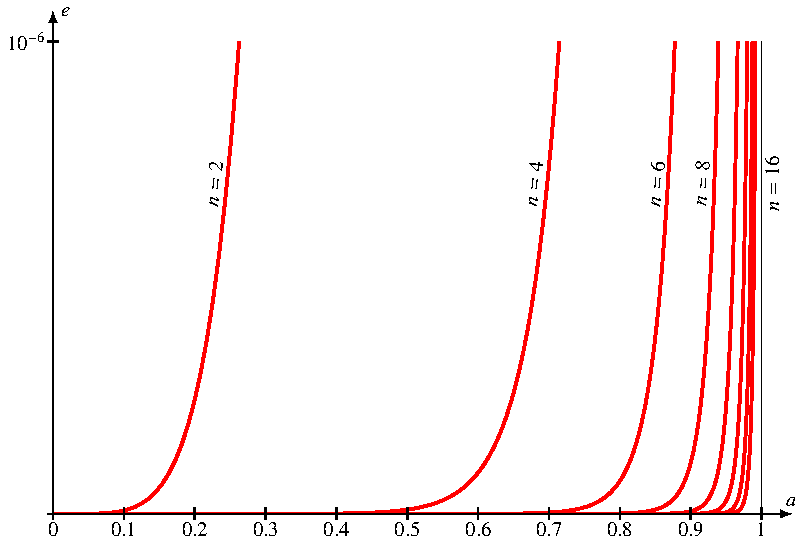
\includegraphics{chapters/060-integral/gq/gq.pdf}
\caption{Approximationsfehler des
Integrals~\eqref{buch:integral:gaussquadratur:bspintegral}
in Abhängigkeit von $a$.
Die Divergenz der Ableitung des Integranden an den Intervallenden
$\pm 1$ führt zu schlechter Konvergenz des Verfahrens, wenn $a$
nahe an $1$ ist.
\label{buch:integral:gaussquadratur:fehler}}
\end{figure}

Zur Illustration der Genauigkeit der Gauss-Quadratur berechnen wir
das Integral
\begin{equation}
\int_{-a}^a \sqrt{1-x^2}\,dx
=
\arcsin a + a \sqrt{1-a^2}
\label{buch:integral:gaussquadratur:bspintegral}
\end{equation}
mit Gauss-Quadratur einerseits und dem Trapezverfahren
andererseits.
Da Gauss-Quadratur mit sehr viel weniger Sützstellen auskommt,
berechnen wir die Trapeznäherung mit zehnmal so vielen Stützstelln.
In den Tabellen~\ref{buch:integral:gaussquadratur:table0.5}
und
\ref{buch:integral:gaussquadratur:table0.999}
sind die Resultate zusammengestellt.
Für $a =\frac12$ zeigt
Tabelle~\ref{buch:integral:gaussquadratur:table0.5}
die sehr schnelle Konvergenz der Gauss-Quadratur, schon mit
12 Stützstellen wird Maschinengenauigkeit erreicht.
Das Trapezverfahren dagegen erreicht auch mit 200 Stützstellen nur
4 korrekte Nachkommastellen.

An den Stellen $x=\pm 1$ divergiert die Ableitung des Integranden
des Integrals \eqref{buch:integral:gaussquadratur:bspintegral}.
Da grösste und kleinste Stützstelle der Gauss-Quadratur immer
deutlich vom Rand des Intervalls entfernt ist, kann das Verfahren
diese ``schwierigen'' Stellen nicht erkennen.
Tabelle~\ref{buch:integral:gaussquadratur:table0.999} zeigt, wie
die Konvergenz des Verfahrens in diesem Fall sehr viel schlechter ist.
Dies zeigt auch der Graph in
Abbildung~\ref{buch:integral:gaussquadratur:fehler}.

\subsection{Skalarprodukte mit Gewichtsfunktion}
Die Nullstellen der Legendre-Polynome ergaben ein gutes
Integrationsverfahren für Polynome auf einem beschränkten
Intervall.
Die Beispiele haben aber auch gezeigt, dass Stellen, wo die
Ableitung des Integranden divergiert, die Genauigkeit stark
beeinträchtigen können.
Ausserdem ist das Verfahren nicht anwendbar auf uneigentliche
Integrale.

\subsubsection{Umgang mit Singularitäten}
Die Lösung des Problems mit Stellen mit divergenter Ableitung
besteht darin, die Stützstellen in der Nähe dieser Stellen
zu konzentrieren.
Die Verwendung einer Gewichtsfunktion $w(x)$ kann genau dies
erreichen.
Statt das Integral einer Funktion $f(x)$ zu bestimmen, 
kann man $f(x)=g(x)w(x)$ schreiben, wobei $w(x)$ so
gewählt werden soll, dass das Verhalten der Steigung an
den Intervallenden gut wiedergibt.
Dies ist mit einer Jacobischen Gewichtsfunktion immer möglich.
Statt der Nullstellen der Legendre-Polynome sind dann die
Nullstellen der Jacobi-Polynome  und die Funktionswete von $g(x)$
an diesen Stellen zu verwenden,  die Gewichte sind
die Integrale von $l_i(x) P^{(\alpha,\beta)}(x)$.

\subsubsection{Uneigentliche Integrale}
Die Berechnung eines uneigentlichen Integrals auf dem Intervall
$(0,\infty)$ oder $(-\infty,\infty)$ ist aus mehreren Gründen nicht
direkt mit dem früher beschriebenen Gauss-Quadraturverfahren
möglich.

Die Stützstellen, die bei der Gauss-Quadratur in einem Intervall
$(a,b)$ verwendet werden, entstehen dadurch, dass man die Nullstellen
der Legendre-Polynome in $(-1,1)$ auf das Intervall $(a,b)$
skaliert.
Dies führt offensichtlich nicht zum Erfolg, wenn ein oder beide
Intervallgrenzen unendlich sind.
Dieses Problem kann dadurch gelöst werden, dass man das unendliche
Intervall $(a,\infty)$ mit
\[
x =  a + \frac{1-t}{t}
\]
auf das Intervall $[0,1]$ transformiert.

Will man beim Intervall $(0,\infty)$ bleiben, dann ist zu beachten,
dass das Integral eines Polynomes immer divergent ist, es ist also
auf jeden Fall nötig, den Integranden durch Funktionen zu approximieren,
die genügend schnell gegen $0$ gehen.
Polynome beliebigen Grades können verwendet werden, wenn sie mit
einer Funktion multipliziert werden, die schneller als jedes Polynom
gegen $0$ geht, so dass das Integral immer noch konvergiert.
Die Funktionen $e^{-x}$ für das Intervall $(0,\infty)$ oder
$e^{-x^2}$ für das Intervall $(-\infty,\infty)$ kommen dafür in Frage.

Um das Integral von $f(x)$ im Intervall $(0,\infty)$ zu berechnen,
schreibt man daher zunächst
\[
\int_0^\infty f(x)\,dx
=
\int_0^\infty g(x)e^{-x}\,dx
=
\int_0^\infty g(x) w(x)\,dx
\quad\text{mit}\quad
w(x)=e^{-x}
\text{ und }
g(x)=f(x)e^x.
\]
Dann approximiert $g(x)$ man durch ein Interpolationspolynom,
so wie man das bei der Gauss-Quadratur gemacht hat.
Als Stützstellen müssen dazu die Nullstellen der Laguerre-Polynome
verwendet werden.
Als Gewichte $w_i$ sind die Integrale der $l_i(x)e^{-x}$
zu verwenden.





